% Toy example of tail blindness and of grouping RR sets by world.  Compile with pdfLaTeX.
% Style of the earlier draft figure: Times text and Computer Modern math (as in the paper), italic panel
% titles, square RR-set cells (blue = S hits the RR set, light gray = miss), orange braces under the worlds.
% Drawn at 1.25x the column width (11.11 cm) with 10/9/8 pt text and included at \columnwidth (scale 0.8),
% so the printed sizes are 8/7.2/6.4 pt but in the lighter 10/9/8 pt Computer Modern designs (no heavy small sizes).
% Numbers: n = 10, 12 RR sets in both sketches, S hits 6 of them.
%   (a) one world per RR set:           sigma_hat = 10 * 6/12 = 5, nothing else is identifiable.
%   (b) 3 worlds, b = 4 RR sets each:   hits 4, 2, 0 -> X_hat = 10, 5, 0; mean 5; CVaR_{1/3} = 0.
\documentclass[border=0pt]{standalone}
\usepackage{times}            % Times text, Computer Modern math, as in IEEEtran
\usepackage{amsmath}
\usepackage{tikz}
\usetikzlibrary{decorations.pathreplacing}
\DeclareMathOperator{\CVaR}{CVaR}

\definecolor{hitc}{HTML}{2A78D6}\definecolor{hitd}{HTML}{256CC0}
\definecolor{missc}{HTML}{E4E3DF}\definecolor{missd}{HTML}{B7B5B1}
\definecolor{brc}{HTML}{F08D65}
\definecolor{gry}{HTML}{5A5A5A}

\tikzset{
  every node/.style={inner sep=0.6pt, text=black},
  ttl/.style={font=\fontsize{10}{12}\selectfont\itshape, anchor=west},
  res/.style={font=\fontsize{10}{12}\selectfont, anchor=west},
  sm/.style={font=\fontsize{8}{9.4}\selectfont, text=gry},
  lab/.style={font=\fontsize{9}{10.8}\selectfont},
  hit/.style={draw=hitd, fill=hitc, line width=0.375pt, minimum size=0.425cm, inner sep=0pt},
  miss/.style={draw=missd, fill=missc, line width=0.375pt, minimum size=0.425cm, inner sep=0pt},
  br/.style={decorate, decoration={brace, amplitude=3.25pt, mirror}, line width=0.75pt, draw=brc},
}
\newcommand{\cell}[3]{\node[#3] at ({#1},{#2}) {};}  % x y style

\begin{document}
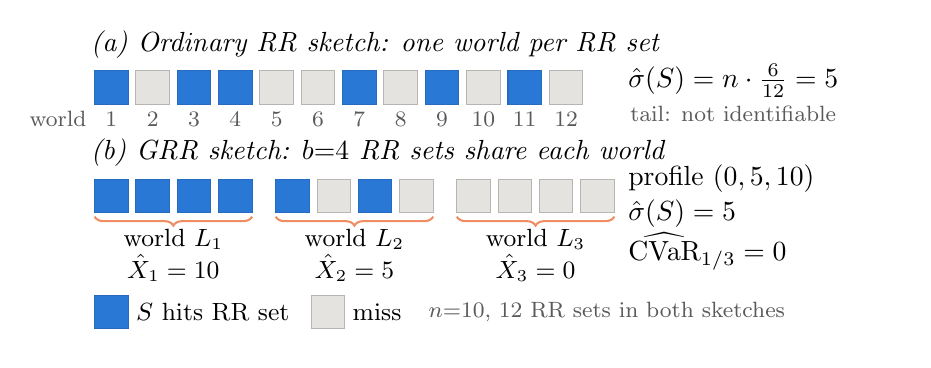
\begin{tikzpicture}[x=1.25cm, y=1.25cm]
\path (0,0.17) rectangle (8.89,-3.00);   % frame: 1.25 x column width

% ---------------- (a) ordinary RR sketch ----------------
\node[ttl] at (0.62,0) {(a) Ordinary RR sketch: one world per RR set};
\foreach \i/\s in {1/hit,2/miss,3/hit,4/hit,5/miss,6/miss,7/hit,8/miss,9/hit,10/miss,11/hit,12/miss} {
  \cell{0.85+(\i-1)*0.42}{-0.44}{\s}
  \node[sm] at ({0.85+(\i-1)*0.42},-0.76) {\i};
}
\node[sm, anchor=east] at (0.62,-0.76) {world};
\node[res] at (6.08,-0.37) {$\hat\sigma(S)=n\cdot\frac{6}{12}=5$};
\node[sm, anchor=west] at (6.10,-0.71) {tail: not identifiable};

% ---------------- (b) GRR sketch ----------------
\node[ttl] at (0.62,-1.10) {(b) GRR sketch: $b{=}4$ RR sets share each world};
\foreach \i/\s in {1/hit,2/hit,3/hit,4/hit,5/hit,6/miss,7/hit,8/miss,9/miss,10/miss,11/miss,12/miss} {
  \cell{0.85+(\i-1)*0.42+floor((\i-1)/4)*0.16}{-1.54}{\s}
}
\foreach \k/\w/\x in {1/{$L_1$}/{$\hat X_1=10$}, 2/{$L_2$}/{$\hat X_2=5$}, 3/{$L_3$}/{$\hat X_3=0$}} {
  \pgfmathsetmacro{\xa}{0.85+(4*\k-4)*0.42+(\k-1)*0.16-0.17}
  \pgfmathsetmacro{\xb}{0.85+(4*\k-1)*0.42+(\k-1)*0.16+0.17}
  \draw[br] (\xa,-1.75) -- (\xb,-1.75);
  \node[lab] at ({(\xa+\xb)/2},-1.98) {world \w};
  \node[lab] at ({(\xa+\xb)/2},-2.27) {\x};
}
\node[res] at (6.08,-1.36) {profile $(0,5,10)$};
\node[res] at (6.08,-1.72) {$\hat\sigma(S)=5$};
\node[res] at (6.08,-2.10) {$\widehat{\CVaR}_{1/3}=0$};

% ---------------- legend ----------------
\cell{0.85}{-2.72}{hit}  \node[lab, anchor=west] at (1.08,-2.72) {$S$ hits RR set};
\cell{3.05}{-2.72}{miss} \node[lab, anchor=west] at (3.28,-2.72) {miss};
\node[sm, anchor=west] at (4.05,-2.72) {$n{=}10$, 12 RR sets in both sketches};
\end{tikzpicture}
\end{document}
